\section{Placa de circuito impreso del módulo interior}
\label{app:componentes-interior}

\subsection{Lista de materiales}

\vfill

\begin{table}[H]
\caption{Lista de materiales del módulo interior}
\label{tab:example}
\begin{tabularx}{\textwidth}{cX}
\toprule
\headingc{Cantidad} & \headingc{Descripción} \\
\topruleb
  1 & PCB de prototipado (70mm x 90mm)\\*\midrule
  1 & NodeMCU v3 (ESP8266)\\*\midrule
  1 & Display LCD 16x2 HD44780 1602A\\*\midrule
  1 & Interfaz I2C para 1602A FC-113\\*\midrule
  1 & Botón \textit{push} (normalmente abierto)\\*\midrule
  1 & LED rojo\\*\midrule
  1 & LED amarillo\\*\midrule
  1 & LED verde\\*\midrule
  2 & Resistencia 1 kΩ\\*\midrule
  1 & Resistencia 100 Ω \\*\midrule
  1 & Un zumbador piezoeléctrico\\*\midrule
  1 & Conversor de nivel lógico (3,3v $\leftrightarrow$ 5v)\\*\midrule
  1 & Interruptor de dos posiciones (3 pines)\\*\midrule
 -- & Pines variados\\*\midrule
 -- & Conectores Dupont variados\\*\midrule
 -- & Cables variados\\*\bottomrule
\end{tabularx}
\end{table}

\vfill

\clearpage

\begin{sidewaysfigure}
  \centering
  \includegraphics[width=0.98\columnwidth]{../photos/interior-pieces}
  \caption{Piezas para la construcción del módulo interior}
  \label{fig:interior-pieces}
\end{sidewaysfigure}

\clearpage

\subsection{Diseño de circuito impreso del módulo interior}

\vfill

\begin{figure}[H]
  \centering
  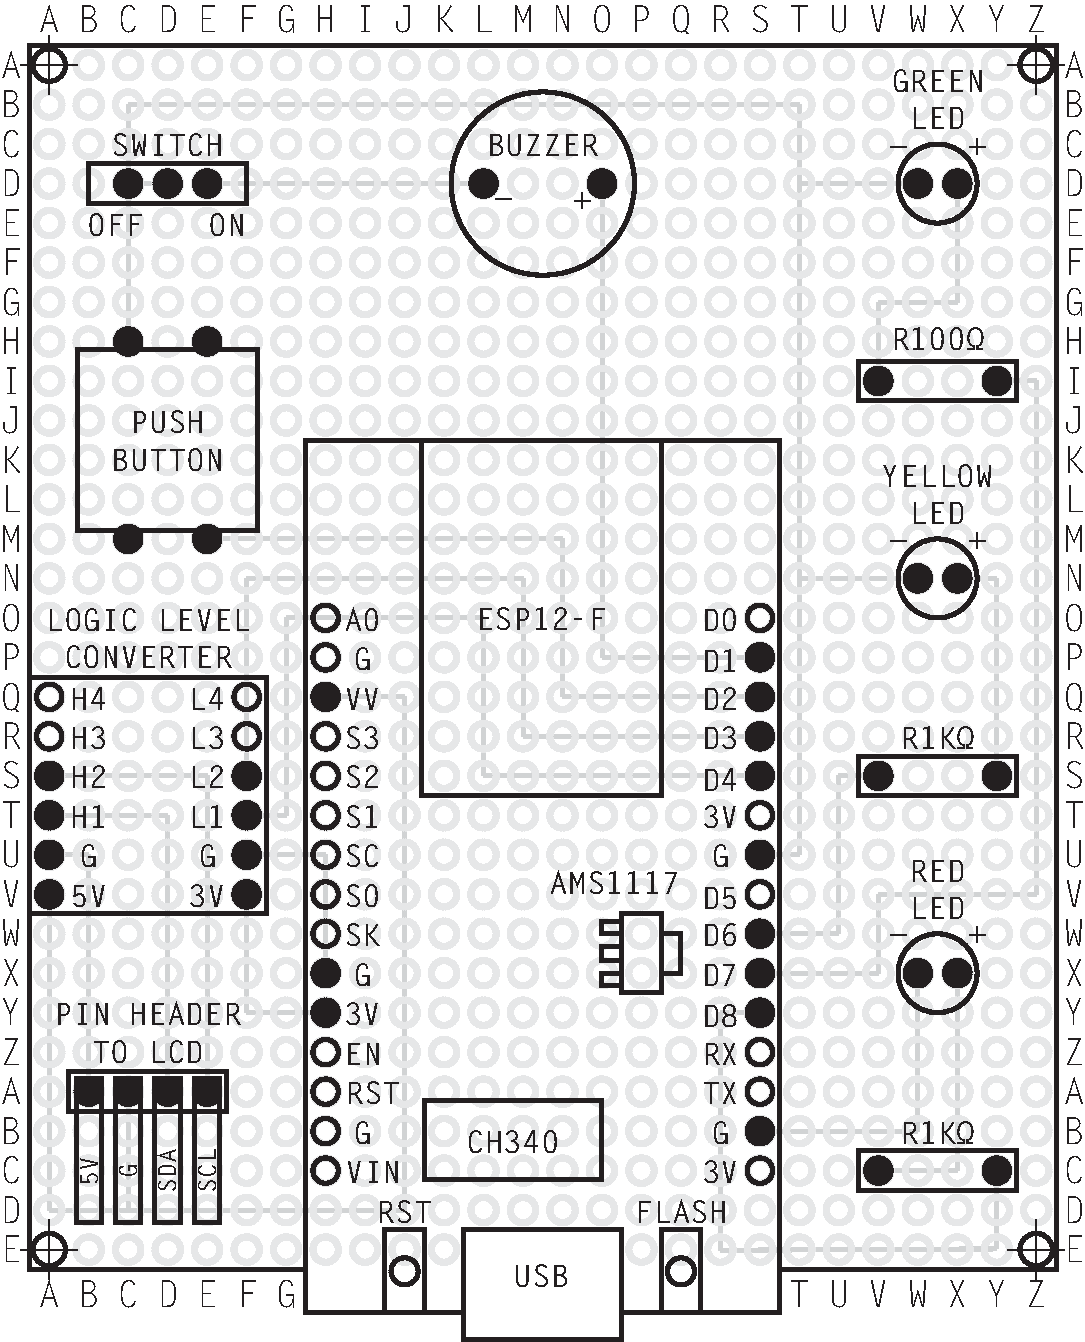
\includegraphics[width=0.7\columnwidth]{../design/interior-board-front}
  \caption{Diseño frontal de la placa de circuito impreso}
  \label{fig:interior-board-front}
\end{figure}

\vfill

\clearpage

\begin{figure}
  \centering
  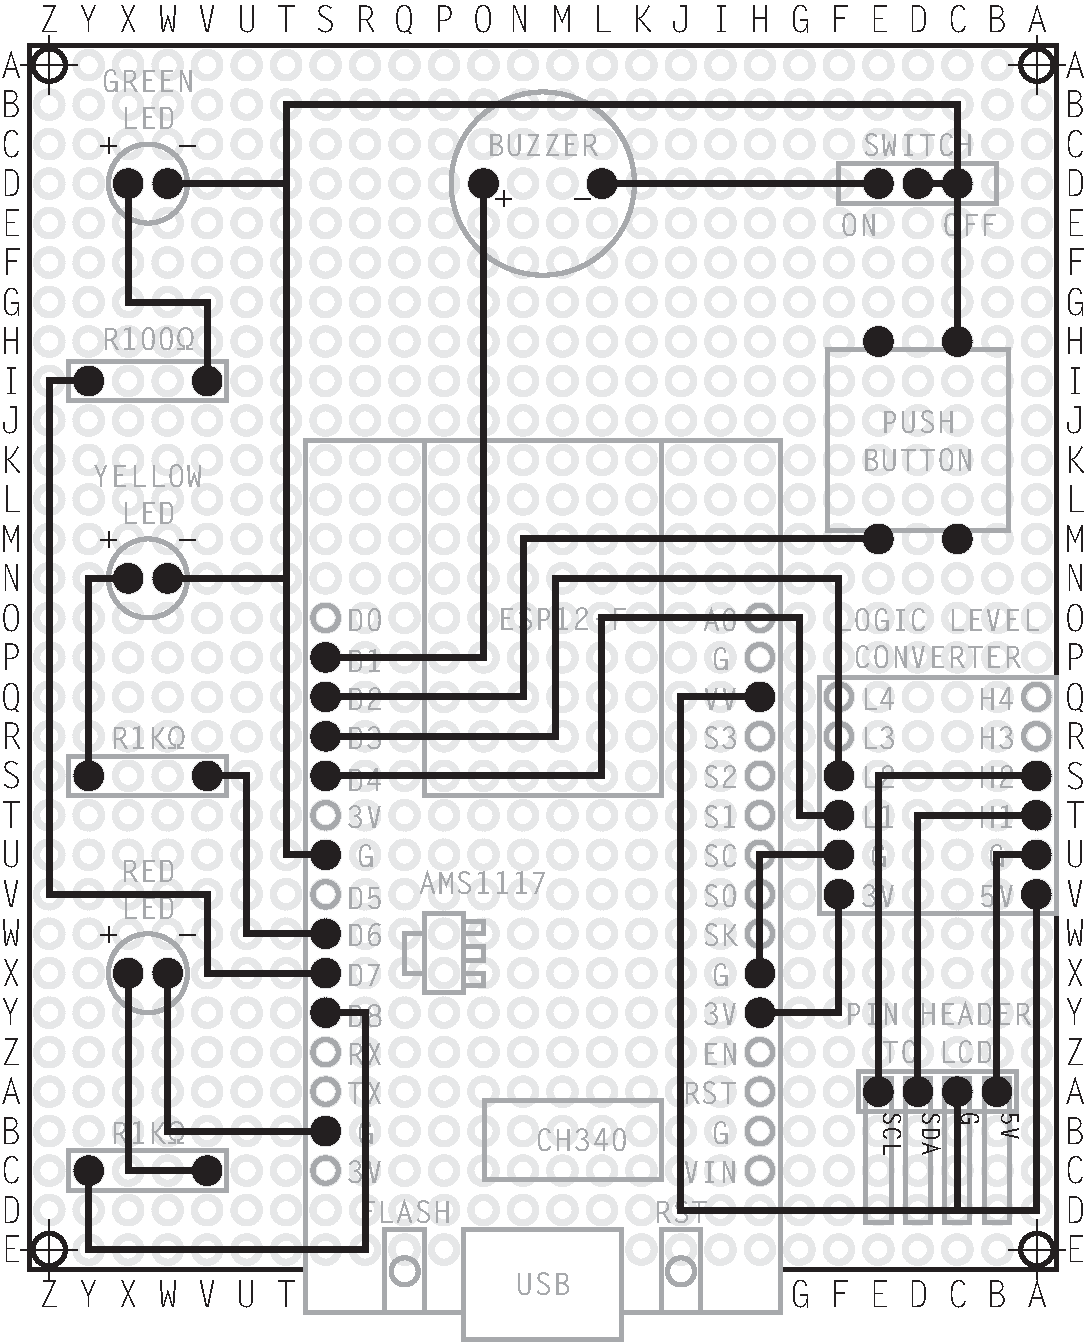
\includegraphics[width=0.7\columnwidth]{../design/interior-board-back}
  \caption{Diseño trasero de la placa de circuito impreso}
  \label{fig:interior-board-back}
\end{figure}

\clearpage

\subsection{Acabado final}

\vfill

\begin{figure}[H]
  \centering
  \includegraphics[width=0.7\columnwidth]{../photos/interior-pcb-front}
  \caption{Acabado final de la placa de circuito impreso (vista frontal)}
  \label{fig:interior-pcb-front}
\end{figure}

\vfill

\clearpage

\begin{figure}
  \centering
  \includegraphics[width=0.7\columnwidth]{../photos/interior-pcb-back}
  \caption{Acabado final de la placa de circuito impreso (vista trasera)}
  \label{fig:interior-pcb-back}
\end{figure}

\clearpage

